\documentclass[aspectratio=169,10pt]{beamer}
\usepackage[utf8]{inputenc}
\usepackage[spanish,es-tabla]{babel}
\usepackage{amsmath,amsfonts,amssymb}
\usepackage{graphicx}
\usepackage{booktabs}
\usepackage{tabularx}
\usepackage{xcolor}

% Tema Beamer limpio y profesional
\usetheme{Madrid}
\usecolortheme{whale}

% Paleta institucional y agrícola tecnológica
\definecolor{unsaacblue}{RGB}{15, 43, 92}
\definecolor{techgreen}{RGB}{16, 185, 129}
\definecolor{darkslate}{RGB}{15, 23, 42}
\definecolor{cardbg}{RGB}{245, 247, 250}

\setbeamercolor{palette primary}{bg=unsaacblue,fg=white}
\setbeamercolor{palette secondary}{bg=techgreen,fg=white}
\setbeamercolor{palette tertiary}{bg=darkslate,fg=white}
\setbeamercolor{structure}{fg=unsaacblue}
\setbeamercolor{titlelike}{parent=palette primary}
\setbeamercolor{block title}{bg=unsaacblue,fg=white}
\setbeamercolor{block body}{bg=cardbg,fg=darkslate}
\setbeamercolor{block title example}{bg=techgreen,fg=white}
\setbeamercolor{block body example}{bg=cardbg,fg=darkslate}

\setbeamertemplate{navigation symbols}{}

\title[Preprocesamiento de Dataset de Imágenes]{\textbf{PREPROCESAMIENTO DE DATASET DE IMÁGENES}}
\subtitle{Detección y Clasificación Temprana de Patologías Foliares en Papa (\textit{Solanum tuberosum}) mediante Visión Artificial}
\author[Y. Supa \& E. Piero Villavicencio]{\textbf{Expositores / Desarrolladores:}\\ SUPA CUSIPAUCAR, Yeferson (220553)\\ VILLAVICENCIO SEGUIL, Edu Piero (220555)}
\institute[UNSAAC]{
    UNIVERSIDAD NACIONAL DE SAN ANTONIO ABAD DEL CUSCO\\
    Facultad de Ingeniería Eléctrica, Electrónica, Informática y Mecánica\\
    Escuela Profesional de Ingeniería Informática y de Sistemas\\[0.2cm]
    \textbf{Docente:} CCACYAHUILLCA BEJAR, HANS HARLEY
}
\date{Octubre 2026}

\begin{document}

% -------------------------------------------------------------------------
% SLIDE 1: PORTADA
% -------------------------------------------------------------------------
\begin{frame}
    \titlepage
\end{frame}

% -------------------------------------------------------------------------
% SLIDE 2: CONTEXTO REGIONAL
% -------------------------------------------------------------------------
\begin{frame}{1. Contexto Regional y Problemática Fitosanitaria}
    \begin{columns}[T]
        \begin{column}{0.48\textwidth}
            \begin{block}{Importancia en Cusco y Andes Peruanos}
                \begin{itemize}
                    \item La papa (\textit{Solanum tuberosum}) es el principal sostén socioeconómico y alimentario regional.
                    \item Pérdidas anuales millonarias por enfermedades criptogámicas foliares.
                    \item Necesidad de diagnóstico temprano y móvil antes de la necrosis total.
                \end{itemize}
            \end{block}
        \end{column}
        
        \begin{column}{0.48\textwidth}
            \begin{exampleblock}{Patologías Foliares Abordadas}
                \begin{itemize}
                    \item \textbf{Tizón Temprano (\textit{Early Blight}):}\\
                    Hongo \textit{Alternaria solani}. Manchas con anillos concéntricos (patrón en diana).
                    \item \textbf{Tizón Tardío (\textit{Late Blight}):}\\
                    Oomiceto \textit{Phytophthora infestans}. Lesiones acuosas rápidas y devastadoras.
                    \item \textbf{Follaje Sano (\textit{Healthy}):}\\
                    Lámina verde sin pústulas (control de referencia).
                \end{itemize}
            \end{exampleblock}
        \end{column}
    \end{columns}
\end{frame}

% -------------------------------------------------------------------------
% SLIDE 3: DATASET DESAFIANTE
% -------------------------------------------------------------------------
\begin{frame}{2. ¿Por qué es un Dataset Altamente Desafiante?}
    \begin{columns}[T]
        \begin{column}{0.48\textwidth}
            \begin{block}{Condiciones de Campo (\textit{In-The-Wild})}
                \begin{itemize}
                    \item \textbf{Iluminación solar extrema:} Luz cenital intensa combinada con sombras arrojadas por hojas superiores.
                    \item \textbf{Reflejos especulares:} Brillos intensos por la cutícula cerosa vegetal.
                    \item \textbf{Fondos heterogéneos:} Presencia de tierra, rastrojos, tallos y superposición foliar.
                \end{itemize}
            \end{block}
        \end{column}
        
        \begin{column}{0.48\textwidth}
            \begin{alertblock}{Retos de Visión Artificial}
                \begin{itemize}
                    \item \textbf{Similitud Inter-Clase Temprana:} En etapas iniciales, las micro-lesiones de \textit{Alternaria} y \textit{Phytophthora} son manchas pardas milimétricas muy parecidas.
                    \item \textbf{Variabilidad de escala y ángulo:} Capturas tomadas manualmente con diversas distancias focales.
                \end{itemize}
            \end{alertblock}
        \end{column}
    \end{columns}
\end{frame}

% -------------------------------------------------------------------------
% SLIDE 4: ARQUITECTURA DEL PIPELINE
% -------------------------------------------------------------------------
\begin{frame}{3. Arquitectura del Pipeline Secuencial}
    \centering
    \begin{tabularx}{\textwidth}{>{\centering\arraybackslash}X >{\centering\arraybackslash}X >{\centering\arraybackslash}X >{\centering\arraybackslash}X >{\centering\arraybackslash}X}
        \toprule
        \textbf{Paso 1} & \textbf{Paso 2} & \textbf{Paso 3} & \textbf{Paso 4} & \textbf{Paso 5} \\
        \midrule
        \textbf{Auditoría de Calidad} & \textbf{Filtrado Bilateral} & \textbf{CLAHE en CIE-Lab} & \textbf{Letterboxing} & \textbf{Particionado \& Augment} \\
        \footnotesize Varianza Laplaciana $\sigma^2 \ge 80.0$ & \footnotesize Denoising no lineal ($d=9, \sigma=75$) & \footnotesize Realce en Luminancia $L^*$ ($8\times8$, clip=2.5) & \footnotesize $256\times256$ con padding simétrico & \footnotesize 70\% Train (Aug), 15\% Val, 15\% Test \\
        \bottomrule
    \end{tabularx}
    \vspace{0.4cm}
    \begin{block}{Principio Fundamental}
        Maximizar la razón señal-ruido y el contraste de micro-lesiones sin introducir deformaciones anatómicas ni sesgos cromáticos.
    \end{block}
\end{frame}

% -------------------------------------------------------------------------
% SLIDE 5: PASO 1 - AUDITORÍA LAPLACIANA
% -------------------------------------------------------------------------
\begin{frame}{4. Paso 1: Auditoría de Nitidez y Desenfoque}
    \begin{columns}[T]
        \begin{column}{0.48\textwidth}
            \begin{block}{Operador Diferencial Laplaciano}
                $$\nabla^2 I = \frac{\partial^2 I}{\partial x^2} + \frac{\partial^2 I}{\partial y^2}$$
                $$\text{Kernel: } K = \begin{bmatrix} 0 & 1 & 0 \\ 1 & -4 & 1 \\ 0 & 1 & 0 \end{bmatrix}$$
                \begin{itemize}
                    \item Las altas frecuencias espaciales indican bordes definidos.
                    \item El desenfoque óptico o de movimiento amortigua drásticamente estas transiciones.
                \end{itemize}
            \end{block}
        \end{column}
        
        \begin{column}{0.48\textwidth}
            \begin{exampleblock}{Métrica de Decisión}
                $$\sigma^2(\nabla^2 I) = \frac{1}{MN}\sum_{x,y}\Big(\nabla^2 I(x,y) - \mu\Big)^2$$
                \begin{itemize}
                    \item \textbf{Imagen Nítida:} $\sigma^2 \ge 80.0$ $\rightarrow$ Apta para modelado.
                    \item \textbf{Imagen Degradada:} $\sigma^2 < 80.0$ $\rightarrow$ Etiquetada como borrosa.
                    \item Evita que la red aprenda patrones falsos por temblor del operario.
                \end{itemize}
            \end{exampleblock}
        \end{column}
    \end{columns}
\end{frame}

% -------------------------------------------------------------------------
% SLIDE 6: PASO 2 - FILTRADO BILATERAL
% -------------------------------------------------------------------------
\begin{frame}{5. Paso 2: Filtrado Bilateral con Preservación de Bordes}
    \begin{columns}[T]
        \begin{column}{0.50\textwidth}
            \begin{block}{Formulación Matemática No Lineal}
                $$I^{\text{filt}}(p) = \frac{1}{W_p}\sum_{q \in \Omega} I(q) \cdot G_{\sigma_s}(\|p-q\|) \cdot G_{\sigma_r}(|I(p)-I(q)|)$$
                \begin{itemize}
                    \item $G_{\sigma_s}$: Distancia euclidiana espacial.
                    \item $G_{\sigma_r}$: Similitud radiométrica de color.
                \end{itemize}
            \end{block}
        \end{column}
        
        \begin{column}{0.46\textwidth}
            \begin{exampleblock}{¿Por qué no Filtro Gaussiano?}
                \begin{itemize}
                    \item El Gaussiano promedia todo el vecindario y difumina los bordes de la lesión.
                    \item \textbf{El Bilateral}: Si $|I(p)-I(q)|$ es grande (borde de mancha marrón vs tejido verde), el peso cae a cero.
                    \item \textbf{Resultado:} Ruido atenuado, bordes y pústulas perfectamente nítidos.
                \end{itemize}
            \end{exampleblock}
        \end{column}
    \end{columns}
\end{frame}

% -------------------------------------------------------------------------
% SLIDE 7: PASO 3 - CLAHE EN CIE-LAB
% -------------------------------------------------------------------------
\begin{frame}{6. Paso 3: Realce Adaptativo CLAHE en Espacio CIE-Lab}
    \begin{columns}[T]
        \begin{column}{0.48\textwidth}
            \begin{block}{¿Por qué en CIE-Lab y no en RGB?}
                \begin{itemize}
                    \item En RGB, la luminosidad está acoplada al tono; ecualizar en RGB distorsiona la clorofila.
                    \item En CIE-Lab se desacopla:
                    \begin{itemize}
                        \item $L^*$: Luminancia perceptual acromática.
                        \item $a^*$: Verde $\leftrightarrow$ Rojo.
                        \item $b^*$: Azul $\leftrightarrow$ Amarillo.
                    \end{itemize}
                    \item Se opera exclusivamente sobre $L^*$.
                \end{itemize}
            \end{block}
        \end{column}
        
        \begin{column}{0.48\textwidth}
            \begin{exampleblock}{CLAHE (Contrast Limited AHE)}
                \begin{itemize}
                    \item \textbf{Teselas Locales ($8\times8$):} Realza contrastes en sombras sin sobreexponer zonas claras.
                    \item \textbf{Clip Limit = 2.5:} Recorta picos de contraste impidiendo amplificar ruido de fondo.
                    \item \textbf{Efecto:} Manchas concéntricas resaltadas preservando el color biológico de la planta.
                \end{itemize}
            \end{exampleblock}
        \end{column}
    \end{columns}
\end{frame}

% -------------------------------------------------------------------------
% SLIDE 8: PASO 4 - LETTERBOXING
% -------------------------------------------------------------------------
\begin{frame}{7. Paso 4: Estandarización Espacial mediante Letterboxing}
    \begin{columns}[T]
        \begin{column}{0.48\textwidth}
            \begin{alertblock}{El Problema del Resize Convencional}
                \begin{itemize}
                    \item Comprime o estira la hoja si el ratio no es 1:1.
                    \item Modifica la circularidad y excentricidad de las manchas de tizón temprano.
                    \item Introduce sesgos geométricos destructivos.
                \end{itemize}
            \end{alertblock}
        \end{column}
        
        \begin{column}{0.48\textwidth}
            \begin{exampleblock}{Solución: Letterbox Isotrópico}
                $$s = \min\left(\frac{256}{W_{\text{orig}}}, \frac{256}{H_{\text{orig}}}\right)$$
                \begin{itemize}
                    \item Escala proporcional uniforme.
                    \item Inserta en lienzo $256 \times 256$ con relleno simétrico negro ($\Delta x, \Delta y$).
                    \item \textbf{Conserva 100\% de la geometría foliar.}
                \end{itemize}
            \end{exampleblock}
        \end{column}
    \end{columns}
\end{frame}

% -------------------------------------------------------------------------
% SLIDE 9: PARTICIONADO Y DATA AUGMENTATION
% -------------------------------------------------------------------------
\begin{frame}{8. Particionado Estratificado y Data Augmentation Riguroso}
    \begin{columns}[T]
        \begin{column}{0.32\textwidth}
            \begin{block}{\centering Train (70\%)}
                \centering \Large \textbf{42 Imágenes}
                \vspace{0.2cm}
                \normalsize
                \begin{itemize}
                    \item Con \textbf{Data Augmentation}.
                    \item Flip horizontal ($p=0.5$).
                    \item Rotación ($\pm 15^\circ$).
                    \item Ajuste fino de brillo y contraste.
                \end{itemize}
            \end{block}
        \end{column}
        
        \begin{column}{0.32\textwidth}
            \begin{exampleblock}{\centering Val (15\%)}
                \centering \Large \textbf{3 Imágenes}
                \vspace{0.2cm}
                \normalsize
                \begin{itemize}
                    \item \textbf{Sin augmentación}.
                    \item Ajuste de hiperparámetros.
                    \item Representa distribución real de campo.
                \end{itemize}
            \end{exampleblock}
        \end{column}
        
        \begin{column}{0.32\textwidth}
            \begin{alertblock}{\centering Test (15\%)}
                \centering \Large \textbf{6 Imágenes}
                \vspace{0.2cm}
                \normalsize
                \begin{itemize}
                    \item \textbf{Sin augmentación}.
                    \item Evaluación final no sesgada.
                    \item Previene fuga de datos (\textit{data leakage}).
                \end{itemize}
            \end{alertblock}
        \end{column}
    \end{columns}
\end{frame}

% -------------------------------------------------------------------------
% SLIDE 10: RESULTADOS EXPERIMENTALES
% -------------------------------------------------------------------------
\begin{frame}{9. Evidencia Experimental del Pipeline}
    \begin{figure}
        \centering
        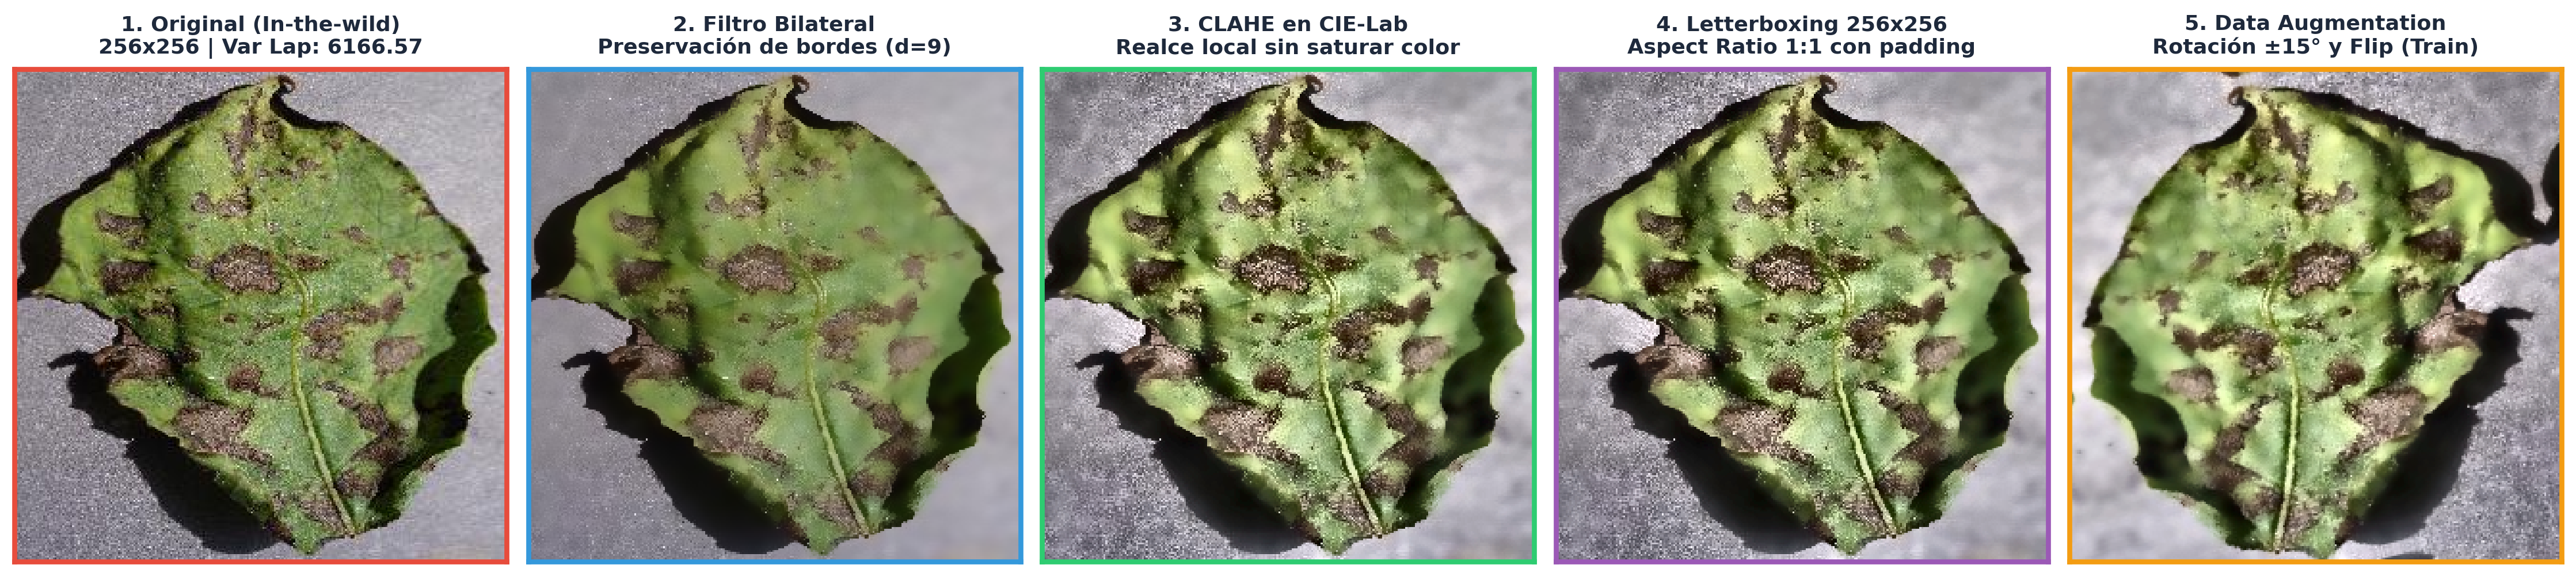
\includegraphics[width=0.95\textwidth]{pipeline_comparativa.png}
        \caption{Evolución visual del pipeline sobre una muestra de \textit{Early Blight}: Original $\rightarrow$ Bilateral $\rightarrow$ CLAHE Lab $\rightarrow$ Letterbox $\rightarrow$ Augment.}
    \end{figure}
\end{frame}

% -------------------------------------------------------------------------
% SLIDE 11: PREGUNTAS TÍPICAS
% -------------------------------------------------------------------------
\begin{frame}{10. Preguntas Clave para la Defensa Oral}
    \begin{block}{1. ¿Por qué no una ecualización global estándar?}
        \small La ecualización global incrementa el contraste acumulado en toda la escena, sobreexponiendo fondos claros y amplificando ruido en áreas lisas. CLAHE limita la amplificación en cuadrículas locales $8\times8$.
    \end{block}
    
    \begin{exampleblock}{2. ¿Por qué Data Augmentation únicamente en Train?}
        \small Validación y Test deben evaluar el modelo frente a imágenes empíricas reales. Aumentar Val o Test provocaría fuga de datos y métricas optimistas falsas.
    \end{exampleblock}
    
    \begin{block}{3. ¿Por qué Letterbox y no simple resize?}
        \small El resize ordinario aplasta o estira las hojas modificando la relación de aspecto y distorsionando las características morfológicas diagnósticas.
    \end{block}
\end{frame}

% -------------------------------------------------------------------------
% SLIDE 12: CONCLUSIONES
% -------------------------------------------------------------------------
\begin{frame}{11. Conclusiones y Próximos Pasos (Segunda Entrega)}
    \begin{columns}[T]
        \begin{column}{0.48\textwidth}
            \begin{block}{Logros de la Primera Entrega}
                \begin{itemize}
                    \item Pipeline automatizado, reproducible y desacoplado en Python/OpenCV.
                    \item Preservación estricta de bordes y geometría foliar mediante Bilateral y Letterbox.
                    \item Particionado estratificado y dataset auditado listo para entrenamiento.
                \end{itemize}
            \end{block}
        \end{column}
        
        \begin{column}{0.48\textwidth}
            \begin{exampleblock}{Segunda Entrega: Modelado y Clasificación}
                \begin{itemize}
                    \item \textbf{Extracción de descriptores:} Textura GLCM (Haralick), momentos de Hu y gradientes de color.
                    \item \textbf{Modelos Deep Learning:} Redes convolucionales livianas (MobileNetV3 y ResNet18) optimizadas para inferencia en campo.
                \end{itemize}
            \end{exampleblock}
        \end{column}
    \end{columns}
    \vspace{0.4cm}
    \centering
    \textbf{\Large ¡Muchas gracias!}
\end{frame}

\end{document}
